\section{Material demoted from the results sections}\label{supp:demoted}

\subsection{Registration: refiling propensity}

Refiling after abandonment is itself mildly related to vocabulary
position, though not on the axis registration responds to: refiling rates
are flat in atypicality (a middle-minus-tails difference of $-0.06$pp on
a 3.6\% base) and rise with lead, from 2.6\% among the most lagging
abandoned applications to 3.4\% among the most leading.

\subsection{The five-year proof: timing, ties, and per-class extremes}

The five-year proof is close to a fixed appointment rather than a hazard
spread over years: of the 1.35 million cancellations recorded for fully
observed cohorts, 17 post before registration age 6.5, 96.1\% post
between 6.5 and 7.0, and the rest after seven. Since the cancellation
record ends on 2 April 2026, a cohort is observable only once it has
reached seven years, which makes 2019 the last one with usable data at
this proof and leaves 2020 and later unobserved. On the 3.15 million
registrations whose ninth anniversary is inside the record --- for which
failure is settled and no window is needed --- the contrast is $+2.71$pp
within class and registration year, against $+2.65$pp on the paper's
4.0--8.5 window; conditional on failing, the probability of failing late
carries a contrast of $-0.01$pp ($t = -0.2$). Response speed does not
predict the outcome: across the 1.22 million scored registrations with a
usable office-action/response pair, passage varies between 46.1\% and
48.1\% across response-speed quintiles, from a median of seven days to
183, and the quickest responders pass slightly \emph{less}; the lead
penalty is present in both halves ($-3.48 \pm 0.40$ and
$-2.36 \pm 0.40$pp on passing, against $-2.94$ pooled). The restriction
drops 61\% of the sample, disproportionately applications that never drew
a refusal.

Tied scores: within the class$\times$registration-year cell the quintiles
are cut in, $17.1$\% of scored registrations share a lead value with at
least one other filing, and the largest tie group runs to 53. Filings
that share a class, a filing date and a goods/services description have
identical distributions scored against identical references. Cut points
are fixed by sorting on the score and then on the serial number; sorting
ties the opposite way moves the top-versus-bottom contrast by $0.001$pp,
and five pseudorandom orderings move it by at most $0.002$pp, against a
contrast of $2.287$pp.

At the year-ten renewal, fitted over 872{,}079 five-year survivors with a
resolved status, a straight line through renewal against lead explains
1\% of the variation across forty bins and a V explains 89\%
($\Delta$AIC $= 83$); renewal peaks at 64.2\% near $z = -0.4$ and falls
to 45.5\% at the most lagging bin and 50.6\% at the most leading. In the
software class, where the five-year lift on the 2010--2013 cohorts
reaches $+12.1$pp, the conditional lift at the renewal falls to
$+7.6$pp.

Per class, the largest raw penalties sit in tobacco ($+26$pp, the vaping
era), hand tools ($+10$pp), processed foods ($+10$pp) and medical
apparatus ($+9$pp), with negative lifts in beer and soft drinks,
transport and construction; these are the extremes of a 44-class screen,
sitting away from zero partly by selection.

\subsection{Waves: the theme tour, internet convergence, and surges}

In 1995--1999 the computer, software, information and data services theme
failed at 64.9\% against 47.5--59.0\% in the other large themes. In
2000--2004 it held 12\% of the leading fifth; the leading language had
moved to video, music and games on electronic media (31\% of the leading
fifth against 12\% of filings), and inside several themes the lagging
fifth failed more than the leading one: $-3.6$pp in electronic media,
$-5.5$ in retail store services, $-6.9$ in apparatus and control systems.
From 2008 the leading fifth over-represented downloadable and online
software 15\% against 4\%; the theme's within-theme contrast cut inside
the 2008--2014 era alone is $+3.3$pp, and the computer-services theme's
own contrast is positive in every era ($+3.6$ to $+5.9$pp) and never
reverses.

The internet gap in event time (Figure~\ref{fig:webshape}): dating the
internet's arrival in each class as the first filing year the pattern
reaches 2\% of the class's filings (1994--1995 in the technology and
transport classes, 1999--2000 in apparel and chemicals, 2008 in
machinery), the gap between internet-bearing registrations and the rest
starts near $+7$ points, declines to about zero nine to eleven years
after arrival, and settles between $+1$ and $+4$; across the eight
classes observable in both phases the mean gap is $+4.4$ points in years
zero to four and $+1.6$ from year ten, shrinking in six of the eight.
Calendar time disguises this: transport (arrival 1995) peaks at $+16$
points in its 2000 cohort; machinery (arrival 2008) peaks at $+17$ in its
2012--2015 cohorts. Clothing is the standing exception: its
internet-bearing registrations outlast the class in every cohort after
2004. Table~\ref{tab:internetS} tabulates the per-class rates.

\begin{figure}[h]\centering
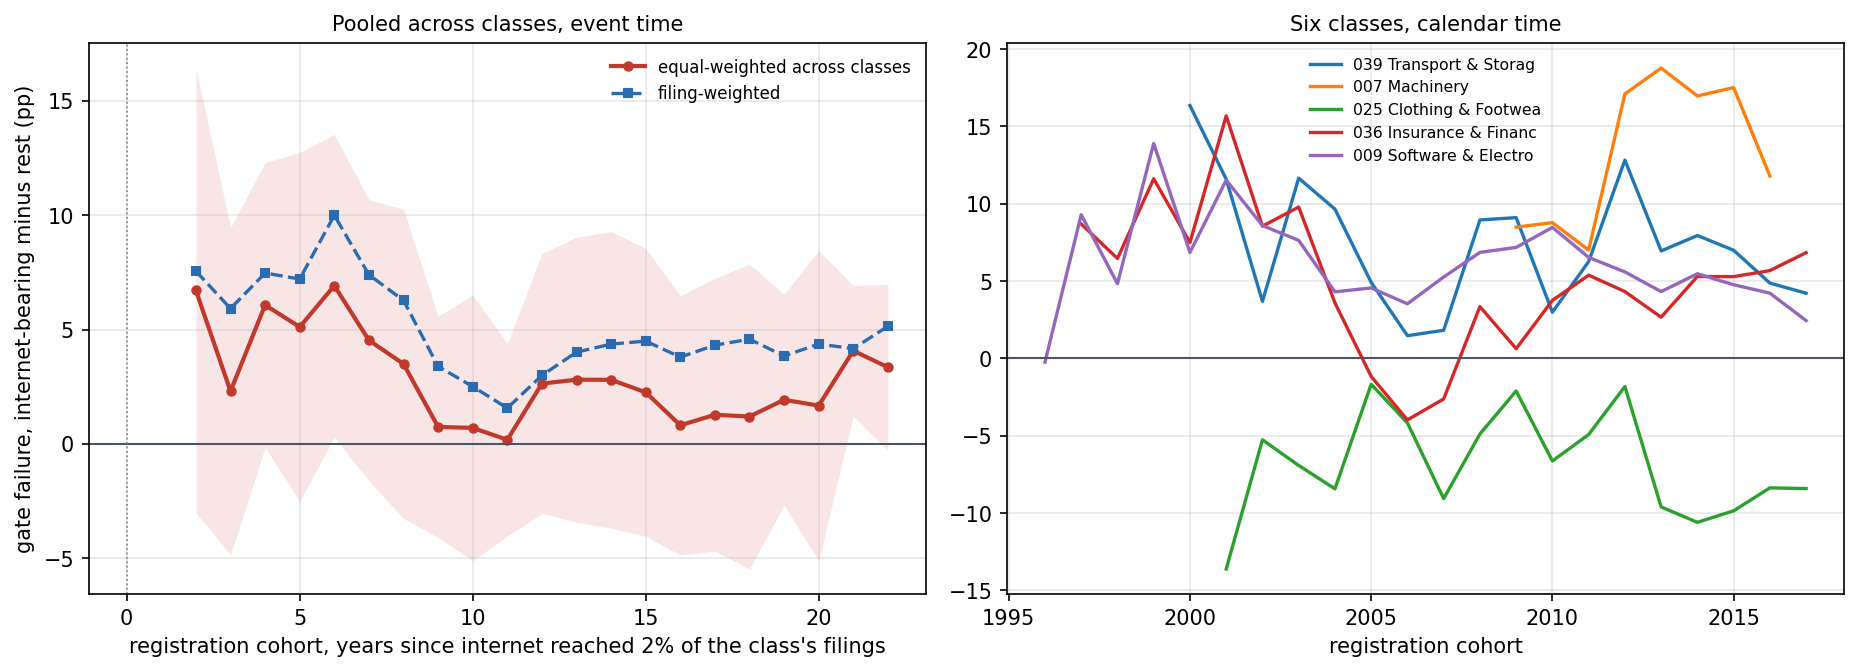
\includegraphics[width=\textwidth]{results/internet_convergence.png}
\caption{The internet gap in failure at the five-year proof, inside each
class. \emph{Left:} internet-bearing minus other registrations' failure
rate, by registration cohort in years since the internet pattern reached
2\% of the class's filings, averaged across classes (band: one standard
deviation across classes). \emph{Right:} five classes in calendar time.
Cells with fewer than 100 registrations in either group are dropped.}
\label{fig:webshape}
\end{figure}

\begin{table}[h]\centering\footnotesize
\caption{Internet-bearing filings against the rest of their Nice class.
Registration is the share of class-records filed 1995--2018 that reached
registration; failure is the share of unique registrations 2002--2018
cancelled for non-use at age 4.0--8.5 years. Classes with fewer than 500
internet-bearing registrations are omitted.}
\label{tab:internetS}
\begin{tabular}{llrrrrr}
\toprule
Class & & Web share & \multicolumn{2}{c}{Registration (\%)} & \multicolumn{2}{c}{Gate failure (\%)} \\
 & & (\%) & web & rest & web & rest \\
\midrule
001 & Chemicals & 1.8 & 65.0 & 64.3 & 46.1 & 39.1 \\
003 & Cosmetics \& Cleaning & 2.8 & 58.0 & 54.2 & 52.1 & 54.4 \\
004 & Lubricants \& Fuels & 4.6 & 63.8 & 56.3 & 50.9 & 47.9 \\
005 & Pharmaceuticals & 1.9 & 53.3 & 48.6 & 52.4 & 53.5 \\
006 & Metal Goods & 3.5 & 68.1 & 67.0 & 44.5 & 39.1 \\
007 & Machinery & 2.8 & 73.3 & 69.7 & 50.9 & 38.7 \\
008 & Hand Tools & 3.6 & 65.8 & 62.5 & 42.4 & 43.6 \\
009 & Software \& Electronics & 18.7 & 53.3 & 57.0 & 56.5 & 51.4 \\
010 & Medical Apparatus & 3.0 & 59.8 & 58.4 & 51.7 & 45.4 \\
011 & Lighting \& Heating & 3.0 & 67.4 & 64.8 & 51.4 & 45.9 \\
012 & Vehicles & 3.4 & 69.0 & 60.9 & 49.6 & 45.1 \\
014 & Jewelry & 7.4 & 63.2 & 55.8 & 54.7 & 55.7 \\
016 & Paper \& Printed Goods & 15.1 & 57.8 & 56.1 & 47.9 & 50.7 \\
017 & Rubber \& Plastics & 2.2 & 70.7 & 67.6 & 44.1 & 38.5 \\
018 & Leather Goods & 8.0 & 61.4 & 57.4 & 50.5 & 55.4 \\
019 & Building Materials & 2.0 & 71.4 & 64.0 & 47.5 & 43.9 \\
020 & Furniture & 4.2 & 62.2 & 59.2 & 47.0 & 48.7 \\
021 & Household Utensils & 5.1 & 60.1 & 59.0 & 44.5 & 50.5 \\
024 & Textiles & 6.0 & 62.8 & 55.9 & 49.7 & 51.2 \\
025 & Clothing \& Footwear & 5.6 & 56.1 & 49.6 & 52.4 & 58.7 \\
026 & Lace \& Embroidery & 7.6 & 61.2 & 55.7 & 52.0 & 53.9 \\
027 & Carpets & 5.6 & 66.8 & 56.8 & 43.7 & 46.9 \\
028 & Games \& Sporting Goods & 6.3 & 55.1 & 53.6 & 54.1 & 55.7 \\
029 & Meats \& Processed Foods & 2.5 & 59.7 & 55.7 & 53.3 & 49.6 \\
030 & Staple Foods & 2.6 & 61.4 & 56.0 & 52.3 & 51.8 \\
031 & Agricultural Products & 2.5 & 60.9 & 58.0 & 49.5 & 43.8 \\
032 & Beer \& Soft Drinks & 2.4 & 58.7 & 49.1 & 56.2 & 53.3 \\
033 & Alcoholic Beverages & 1.2 & 61.3 & 52.7 & 56.9 & 42.3 \\
034 & Tobacco & 2.9 & 53.8 & 49.1 & 55.0 & 54.2 \\
035 & Advertising \& Retail & 40.7 & 59.3 & 61.2 & 57.9 & 52.0 \\
036 & Insurance \& Finance & 18.9 & 58.6 & 62.6 & 52.4 & 48.9 \\
037 & Construction \& Repair & 10.4 & 67.8 & 67.5 & 49.0 & 47.1 \\
038 & Telecommunications & 57.6 & 54.5 & 45.1 & 60.8 & 60.1 \\
039 & Transport \& Storage & 21.3 & 62.5 & 63.1 & 54.8 & 47.6 \\
040 & Material Treatment & 9.6 & 68.0 & 63.9 & 49.4 & 47.3 \\
041 & Education \& Entertainment & 35.0 & 61.1 & 60.6 & 54.2 & 52.5 \\
042 & Scientific \& Tech Services & 39.3 & 57.8 & 59.4 & 58.0 & 51.4 \\
043 & Hotels \& Restaurants & 9.1 & 62.9 & 58.7 & 53.8 & 48.1 \\
044 & Medical \& Beauty Services & 20.6 & 62.9 & 62.1 & 53.7 & 51.3 \\
045 & Legal \& Personal Services & 41.5 & 60.3 & 65.0 & 60.1 & 48.7 \\
\bottomrule
\end{tabular}

\end{table}

Surge episodes (Figure~\ref{fig:surgesS}): measured against the whole
corpus at a 1\% share, five themes ever surge and one clears a
1{,}000-registration floor --- online software, 1999, whose 6{,}339
in-window registrations failed at 63.7\%. Within-class episodes differ in
sign among themselves: the education-services surge in advertising and
retail after 2002 failed $13.7$ points \emph{less} than its class; the
charitable-fundraising surge in finance after 2011 failed $4.0$ points
more; of the episodes large enough to carry their own lead contrast, one
is positive ($+5.8$pp, $t = 2.2$) and the rest indistinguishable from
zero. On the 61 episodes with at least 300 joining registrations over a
six-year entry window (64{,}105 of 86{,}447 joining registrations):
joiners in the surge year fail $-0.8$ points relative to their wave's
mean and joiners five years in $+0.0$, with no gradient between (SEs
$\sim 0.5$); excess failure is $+2.7$, $+3.9$ and $-0.1$ points across
wave-size terciles, correlating with size at $-0.22$; and waves whose
theme share is still at or above its surge level five years on carry
$+4.3$ points of excess against $+1.0$ for receding waves.

\begin{figure}[h]\centering
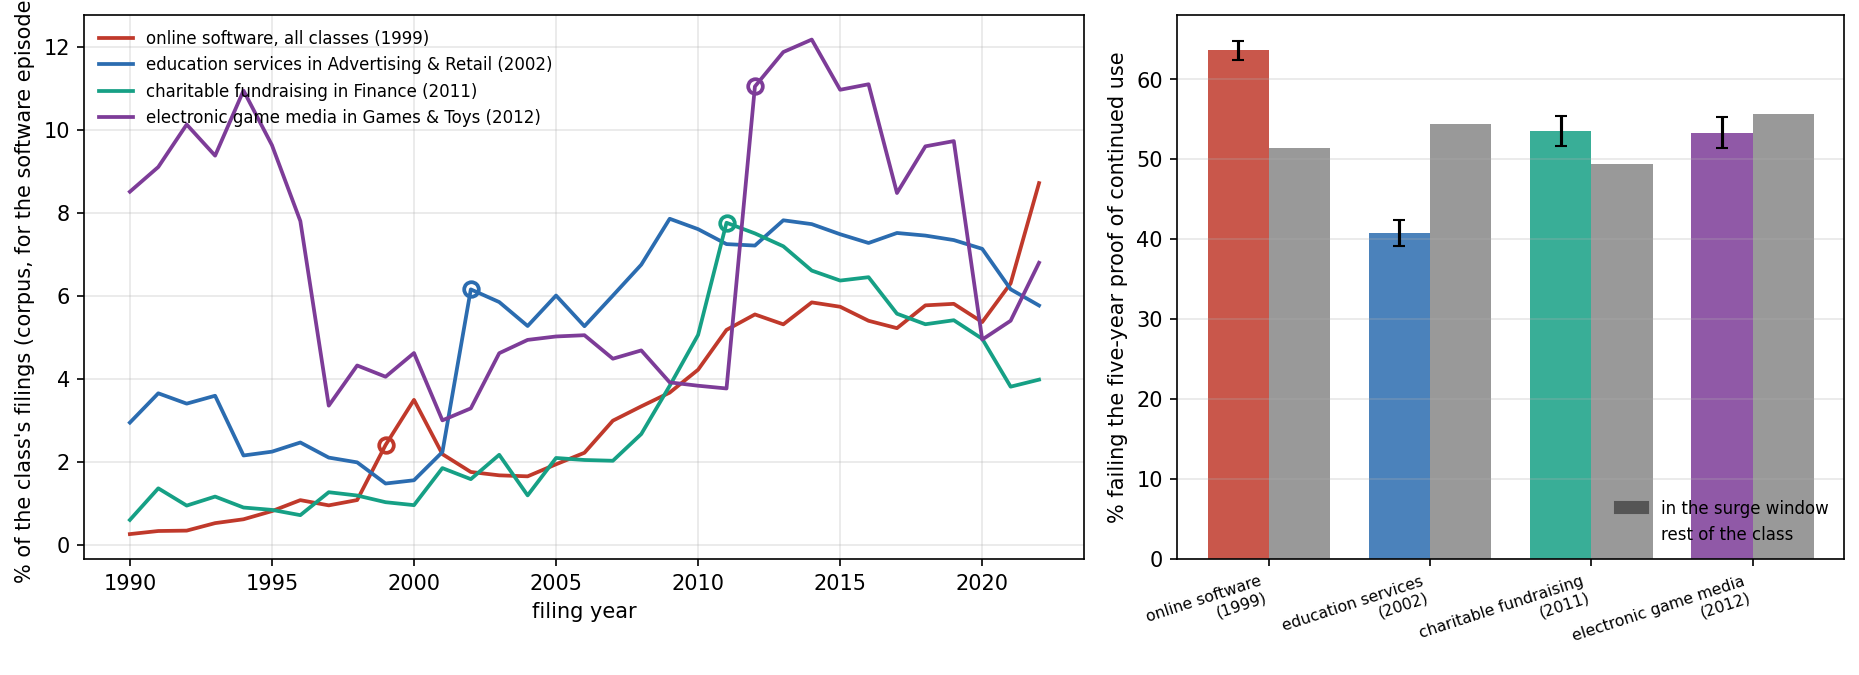
\includegraphics[width=\textwidth]{results/fig_surges.png}
\caption{Four surge episodes under the 500-theme model. \emph{Left:} the
theme's share of its class's filings by filing year (for the online
software episode, of all filings corpus-wide), on the 25\% systematic
sample the surge screen uses; the open circle marks the surge year.
\emph{Right:} failure at the five-year proof for registrations whose
dominant theme was the surging one, filed in the three-year surge window
(colored, 95\% intervals), against the rest of the same class in the same
cohorts (grey).}
\label{fig:surgesS}
\end{figure}

\subsection{Success: the unfunded listings, the value tiers, and the curated vocabularies}

Of the 1{,}669 debut owners with an IPO marker, 759 have no post-debut
Form D round in the record; their debut lead averages $-0.22$ standard
deviations (SE $0.04$) against $-0.07$ (SE $0.04$) for the 910 funded,
29\% sit in the most lagging fifth against 22\%, and both groups are
mildly atypical ($+0.13$ and $+0.15$). Rounds before 2009, foreign
placements, and registered offerings post no Form D.

Value tiers: ten linked owners hold 18.5\% of \$19.2 trillion of linked
peak revenue, fifty hold 41.5\%, a hundred 53.6\%, five hundred 82.9\%,
a thousand 92.6\%. The ten largest sit $0.35$ standard deviations below
average atypicality and within $0.01$ of average lead; the fifty largest
$0.08$ below and $0.13$ above; the five hundred largest within about
$0.1$ on both; revenue-weighting the whole linked set gives $-0.02$ and
$0.00$.

Curated vocabularies: internet wording appears in 2.94 million
class-filing rows, AI in 167 thousand, blockchain in 114 thousand;
registration rates are 52.1\%, 34.5\% and 31.2\% against 57.6\% for all
debut filings (the last two cohorts are young). On the 2009--2018 ladder
under the rebuilt Form D match, AI debuts are funded at 7.8\% and
blockchain at 8.0\% against 2.8\% for internet and 1.6\% overall, while
at the IPO rung the gap disappears: 0.16\% of AI debuts, 0.22\% of
blockchain, and 0.21\% of internet debuts against 0.17\% overall
(1{,}896 AI debuts, 1{,}366 blockchain).

Patent sector split: on the coarse complements/substitutes sorting
(eleven complement classes assigned from class definitions; sectoral
build at 200 themes, firms with at least three panel years, 50 firms and
300 firm-years per cell), complement classes run from sixth to
twenty-fourth of 27 by coefficient and disagree in sign; the only
significant cells are paper and housewares, both negative, neither a
complement class; on the wider 34-class retention the significant
positives are transport and cosmetics and the significant negatives
include medical devices and machinery.

\subsection{The measure: Amazon's theme shares and the length null}

Of the six themes Amazon's 1997 filing drew on, the share of class-035
filings drawing on each in the five years before and after: retail store
services $42.6 \to 50.3$\%, computer and information services
$58.9 \to 59.9$, media and entertainment goods $9.9 \to 11.3$,
downloadable and online software $2.3 \to 4.1$, printed matter
$8.3 \to 7.8$, marketing of consumer goods $10.5 \to 9.3$ (a theme counts
as drawn on at a tenth of the filing's weight or more). Synthetic filings
whose words are drawn at random from the reference itself, maximally
ordinary by construction, score $5.72$ nats at three tokens and $1.65$ at
four hundred, tracking $\log(\text{distinct terms})$ to within a fiftieth
of a nat; the average real filing scores marginally below that null at
its own length. The theme-pair windows behind the pair-lead measure are
calendar-year buckets scored only when they hold at least 2{,}000
filings; word-level recombination counts adjacent pairs appearing fewer
than five times in the class's prior five years while both words appear
at least fifty times, with the share taken over such eligible pairs; the
raw top-versus-bottom recombination contrast is $6.1$ points before the
lead and atypicality controls reduce it to $2.8$.